% This is based on the LLNCS.DEM the demonstration file of
% the LaTeX macro package from Springer-Verlag
% for Lecture Notes in Computer Science,
% version 2.4 for LaTeX2e as of 16. April 2010
%
% See http://www.springer.com/computer/lncs/lncs+authors?SGWID=0-40209-0-0-0
% for the full guidelines.
%

\documentclass{llncs}

\usepackage{hyperref}
\usepackage{subcaption}
\usepackage[]{todonotes}
%\def\includegraphic{}
%\def\includegraphics{}
\usepackage{graphicx}

\usepackage{url}
\usepackage{fancyhdr}
\usepackage{lastpage}
\pagestyle{fancy}
\fancyhf{}
\rfoot{Page \thepage \hspace{1pt} of \pageref{LastPage}}

\captionsetup{compatibility=false}
\setlength{\tabcolsep}{8pt}
\hypersetup{
  colorlinks   = true    % Colours links instead of ugly boxes
}

\begin{document}

\title{Semantic social networks: a new approach to scaling digital ethnography}
%
\titlerunning{Semantic social networks}  % abbreviated title (for running head)
%                                     also used for the TOC unless
%                                     \toctitle is used
%
\author{Alberto Cottica\inst{1} \and Amelia Hassoun\inst{2} \and Jason Vallet\inst{3}  \and Guy Melan{\c{c}}on\inst{3}}
%
\authorrunning{A. Cottica et al.} % abbreviated author list (for running head)
%
%%%% list of authors for the TOC (use if author list has to be modified)
\tocauthor{Alberto Cottica, Jason Vallet, Amelia Hassoun, Guy Melan{\c{c}}on}
%
\institute{Edgeryders, EE; University of Alicante, SP\\
\email{alberto@edgeryders.eu},\\ 
% WWW home page: \texttt{http://edgeryders.eu}
\and
University of Oxford, UK
\and
Universit\'{e} de Bordeaux,
CNRS UMR 5800 LaBRI, FR}

\maketitle              % typeset the title of the contribution

\begin{abstract}
We propose a data-based approach to doing ethnographic research in a digital environment. It has three main components. First, it treats online conversational environments as human communities that ethnographers can engage with as they would in onsite fieldwork. Second, it represents those conversations and the fieldnotes made by researchers thereon in network form. e call these networks \emph{semantic social networks}, as they incorporate information on social interaction and their meaning. They encode a map of the associations between key concepts as perceived by informants as a group.  
Third, it uses methods borrowed from network science to process these data. 

We present an application of this method to a large online conversation about community provision of health and social care, and discuss its potential for harnessing collective intelligence.
\keywords{digital ethnography, network science, collective intelligence}
\end{abstract}
%
\section{Introduction} \label{sec_introduction}


The Internet Age has brought about a wave of exploration and innovation into digital ethnographic research methods. Substantial work has been devoted to methods that mine social networking platforms for user-generated content to analyse, often automatically.  We propose an alternative approach based on convening an online conversation on the topic of interest. Such conversations function as virtual communities~\cite{Rheingold2000}. As such, they lend themselves to participant observation. 

The digital nature of the conversational medium transforms the ethnographic evidence into structured data. This offers two opportunities. First, it allows ethnographers to do quantitative analysis on their own qualitative analysis. Secondly, as quantitative analysis functions as an aggregation layer, it allows ethnographers to handle larger volumes of evidence in coherent, replicable ways.

In what follows, we show how ethnographic evidence maps onto a type of network that encodes both social interaction and semantic association. We call these networks \emph{semantic social networks (SSNs)}, and claim that a methodology based on them is highly accountable to ethnography as a a discipline. Its steps, save for the final quantitative analysis layer, carry naturally over from onsite field research to the digital domain. So, then, does ethnography's distinctive focus on groups of humans and their worldviews.

Additionally, SSNs are much more scalable than traditional ethnography. Coupled with open data  and open standards, they can work well with thousands of informants – a scale large enough for most applications, and much larger than that achieved by traditional ethnography. In sum, SSNs have the potential to evolve in a research method that (a) discovers \textit{collective} worldviews of groups of humans; (b) can address open questions (unlike surveys) and (c) scales reasonably well (unlike onsite ethnography). They show promise as tools to harness \emph{collective intelligence}, the processing of information by connected groups of humans \cite{levy1997collective}.

\indent In what follows, we describe the approach and present the results obtained by applying it to a digital ethnography dataset. We first introduce a data model for SSNs (section \ref{sec:data:model}). Next, we present data in SSN form from a study on community-provided health and social care services (section \ref{sec_opencare_data}. We then illustrate how we used SSNs to aggregate and navigate a large corpus of ethnographic evidence (section \ref{sec_results}). Finally, we reflect on some possible extensions to SSNs and their potential for allowing digital ethnography to scale, while still maintaining its methodological advantages(section \ref{sec:extensions}). 

% After describing the two approaches along the data collection-data analysis cycle (Sect. \ref{sec_opencare_data}), we present the OpenCare dataset and the process followed to extract the codes assigned by ethnographers (Sect. \ref{sec_materials_methods}). We then analyse the co-occurrences of codes in the form of a graph, to identify contributions referring to similar subjects and compare the results of our analytical method to those returned by an analysis performed on a dataset gathered through social media trawling (Section \ref{sec_results}). Finally, we reflect on these conversational environments and the study of their potential as a methodological tool for future ethnographic work against the backdrop of other available methods for digital ethnography.

\section{Semantic social networks: a generalised data model for digital ethnography: } \label{sec:data:model}

Ethnography is a qualitative research technique aimed at discovering how a certain group of humans perceives a set of issues. Its unique value lies in that its findings encode the culture and worldview of the group being studied. This makes it especially suited for applications like foresight~\cite{barben200838} and democratic stakeholder dialogue~\cite{conley2005engage,wolford2007confusion}, where social and cultural meanings that arise organically from human interactions are the main objects of research rather than pre-conceived, researcher-imposed analytical categories.

Field-based ethnography treats access to informants embedded in communities as its most precious resource~\cite{Geertz1973}. As the discipline expanded in topical scope and methodology, it retained its focus on extracting meaningful information by seeking analytical depth through engagements with relatively small numbers of informants~\cite{Abu-Lughod1991}. This depth is typically achieved in part with long, repeated interviews with informants. Researchers then transcribe the text and associate transcripts to keywords, called \emph{codes}, which form an ontology of concepts relevant to describe the problem at hand. These codes emerge from the ethnographer's embeddedness in the community she studies, gleaned through extended participant-observation which contextualises interview data in informants' larger environment~\cite{Emerson2011,Goffman1989}. 

Confronted with the rise of the global Internet, qualitative social scientists followed two main paths. One consists in mining social networking websites and applying quantitative analysis techniques to the retrieved material (\cite{Munk2016,Hollstein2011}). We do not discuss it here.

The other consists in convening online conversations specifically to debate the issue at hand, and treating those conversations as ethnographic data. In this approach, informants co-construct and sustain visible themes of conversation through interaction with the researcher. Further, when an ethnographer is synchronically doing research with informants, she can contextualise the temporal unfolding of information rather than getting lost in noise as in other methods that analyse aggregated digital data after the fact~\cite{Coleman2010}. This approach relates to works such as participant-observation with UNIX user-groups~\cite{Kelty2008}, online research with Anonymous hackers~\cite{Coleman2015}, and fieldwork in virtual worlds like World of Warcraft~\cite{Nardi2010} and Second Life~\cite{Boellstorff2008}. In these studies, anthropologists conducted long-term ethnography, interacting with informants in-setting, asking questions, and generating context-specific data that evolved through interactions with informants over time. Some projects included offline components~\cite{Kelty2008}, while others were completely undertaken online~\cite{Boellstorff2008}, but all pay close attention to the ways informants make sense of their own worlds and define their terminology.

%OpenCare similarly commits to engagement with informants, but also convenes the environment within which conversations unfold. This allows researchers to code data directly on the OpenCare site, resulting in a rich overlay of quantitative data over the qualitative data generated by informants and coded by ethnographers. 

To process ethnographic evidence at scale, we recast it as \emph{data}. Data are characterised by a structure, common to all datapoints in a given dataset, that makes it amenable to being processed by machines. Machine processing, in turn, paves the way to research at scale. The specific challenge for ethnographers is to fit their evidence into a data structure without compromising its rich, contextual character.
In this section, we describe the data structure we implemented in the course of a project called OpenCare.\footnote{\url{http://opencare.cc}} It explores how communities of any kind provide health and social care, when neither states nor business can or will serve them. It consists mostly of an online interaction environment, where individuals share their experiences of care with others, discuss, and compare notes.

\subsection{Primary data: contributions} \label{ssec_primary_data}

SSN-based ethnographies start with the posts/comments on the social networking platform or online forums that hosts the conversation. We call \emph{contribution} a testimony in written form (interview transcript, post on an online forum, etc.). A contribution is a datapoint of the study's primary dataset, the one generated by the informants themselves. A minimum viable structure for encoding a contribution as primary data includes:
\begin{description}
\item[Contribution ID] The contribution's unique identifier.
\item[Text] The contribution's complete text.
\item[Author ID] A unique identifier for the informant that contributed the text. 
\item[Target ID] A unique identifier for the informant that the text is addressed to.
\item[Date and time] 
\end{description}

\subsection{Secondary data: annotations} \label{ssec_secondary_data}
As we noted in section \ref{sec_introduction}, ethnographers work by associating snippets of texts in the primary data to codes (keywords). This generates an ontology representative of the corpus of evidence at hand. In doing so, researchers produce secondary data. We call \emph{annotation} the atomic result of this activity. A minimum viable structure for annotations as secondary data includes:
\begin{description}
\item[Annotation ID] The annotation's unique identifier.
\item[Contribution ID] The unique identifier of the post or comment that this annotation refers to.
\item[Snippet] The part of the text in the contribution that the researcher wishes to associate with the code.
\item[Code] The ethnographic code associated to the snippet.
\item[Author ID] Unique identifier for the researcher that produced the annotation. It is useful in the case of multi-author studies.
\item[Date and time].
\end{description}

This representation is sufficient to induce a network where the nodes are informants, and edges represent interactions. Codes – associated to the interaction via annotations – encode the semantics of that interaction. This is what we call a SSN (Figure \ref{fig:SSN}). It proved to be easy to implement with most forum or blogging software applications;  simple to process in meaningful ways (see below); and scalable. We propose it is general enough to fit the evidence from most ethnographies, while still rigid enough to encode it into well-formed datasets. 

\begin{figure}[h!]
\centering
\includegraphics[scale=0.13]{images/SSN.jpeg}
\caption{An interaction between two informants that carries an ethnographic code id the atom of SSNs.}
\label{fig:SSN}
\end{figure}


%\footnote{This is because it makes very general assumptions about how such software stores primary data. All applications we are aware of use some variant of SQL; information is stored in tables, and referenced by IDs.}
%
% insert Figure 1.
%
%\begin{figure}[h]
%\centering
%\begin{tabular}{ l || c | c|| c | c | c|}
%Network & $N$ & $E$ & $\bar{d}$ & $\bar{C}$ & $\bar{D}$ \\ \hline
%opencare & 990 & 12,777 & 25.81212 & 0.71091 & 2.58182 \\  \hline
%ring lattice & 990 & 12,870 & 0.72 & 19.5197 \\ \hline
%random & 990 & 12,870 & 0.02686 & 2.46629 \\ \hline
%instagram & 2,045 & 23,693 & 23.17164 & 0.83434 & 3.26446 \\ \hline
%ring lattice & 2,045 & 24,540 & 0.717391 & 43.0841 \\ \hline
%random & 2,045 & 24,540 & 0.011982 & 2.73801 \\ \hline
%\end{tabular}
%\caption{Statistics of the analysed network datasets. $N$: number of nodes, $E$: number of edges, $\bar{d}$: average degree ($\bar{d}=2E/N$), $\bar{C}$: average clustering coefficient, $\bar{D}$: average path length.}
%\end{figure}

\section{An application: the OpenCare data} \label{sec_opencare_data}

% TODO: recompute all numbers and draw fresh networks

The OpenCare project explores how communities of any kind provide health and social care, when neither states nor businesses can or will serve them. Data are gathered from an online forum where individuals share and discuss their experiences of community-provided care. At the time of writing, the forum consists of 439 long-form posts with 2,082 comments, authored by 254 unique informants. These were uploaded onto the online forum in the period between January 2016 and May 2017. This corpus was enriched with 4,555 annotations, employing 1,035 unique codes. 

%Each long-form post is used to start a conversation and is submitted by a single author. Posts are commentable and new comments can then be written to either answer directly to the initial post or to be attached to another comment when reacting to it. The resulting structure forms a tree with the initial post as its root and the comments, and comments to comments forming branches. Ethnographers analyse this content and annotate them as described above. 


\subsection{The OpenCare social network} \label{ssec_social_network}

Online conversation in OpenCare induces a social network where nodes are community members, and edges encode interaction. For two users $A$ and $B$, we produce a connection $A \rightarrow B$ if $A$ has commented $B$'s content at least once. This network is directed ($A \rightarrow B \neq B \rightarrow A$) and weighted (the edge $A \rightarrow B$ has a weight of $k$ if $A$ has commented $B$'s content $k$ times). It has 249 nodes and 1,007 edges
The main feature of this network is that there are no signs of polarisation, nor of balkanisation. Almost all participants are connected to the giant component, so that information is allowed to flow freely across the network. The giant component itself is not obviously resolved into distinct sub-communities (the Louvain modularity value is 0.33). These structural features allow us to conditionally accept that most opinions expressed in the forum have been run past someone (other than the proponent) in the conversation.

\subsection{The OpenCare semantic network}

The network representation that proved the most useful to ethnographic research is what we call the \emph{co-occurrence network}. Its nodes are codes. Its edges are induced between two codes that occur in annotations that refer to the same post or content. This network is undirected ($A \rightarrow B \equiv B \rightarrow A$) and weighted (the edge has a weight of $k$ if $A$ co-occurs with $B$ on $k$ different posts or comments).

We can think of the co-occurrence network as an association map between the concepts expressed by the codes. A higher edge weight $k$ indicates a stronger group-level association between the two codes connected by the edge. 

The annotations on the OpenCare corpus induce a co-occurrence network with 1,035 nodes and 12,785 edges. The main component is formed of 990 nodes and 12,777 edges, and is an perfect example of small-world network as defined in~\cite{Watts1998}, with a high average clustering coefficient $\bar{C} = 0.711$.

%The chosen co-occurrence is strictly limited to tags manifesting in the same content, but different levels of precision could be set. For less strict conditions, we could either base the relation between two tags upon the co-occurrence in a direct response (if both tags appear in a content and in an immediate comment on it), an indirect response (tags existing in the same discussion: a response to a response\dots to a content) or simply in the same thread (the tags exist in any of the contents referring to the same initial post). While all these solutions can offer potential insights on the tags and their co-occurrences, each step also brings some noise and meaningless relations. We have thus decided to only use the stricter definition of co-occurrence, linking any two tags co-existing in the same content.

\section{Results and discussion} \label{sec_results}

\subsection{Filtering the co-occurrence network for a high-level view} \label{ssec_filtering_co_occurrence}

We can think of the codes co-occurrence network as a concept association map. Rather than representing the point of view of an individual, it encodes contributions from all informants, since informants are known to be in conversation with each other about the topic at hand. The resulting concept map, therefore, does not simply \emph{aggregate} the association patterns of individuals, like a survey; it is the product of the \emph{interaction} across participants. Edge weight $k$, then, represents the strength with which the conversation (as opposed to its participants) associates the codes connected by that edge. 

Filtering the graph by higher value of $k$ allows the researcher to single out the strongest associations between codes made by the informants as a group. Figure \ref{fig:NetViz} shows the OpenCare code co-occurrence network for $k>=5$ (69 codes, 96 edges). The color coding was generated by applying to it the Louvain community detection algorithm~\cite{blondel2008fast}. It is a highly modular network (modularity = 0.59), with clearly distinguishable groups of codes. This suggests that the debate self-organised into sub-issues.  

Even with no access to the primary data, one can glimpse the structure of the debate among informants. Consider for example the cluster around \texttt{legality} (in blue): we find \texttt{existing system failure} and \texttt{regulation}, reflecting the preoccupation of some informants that community health care initiatives (much needed when systems fail), turn out to be illegal. We also find \texttt{safety}, reflecting the acknowledgement that regulation is there for a reason.

\begin{figure}[h!]
\centering
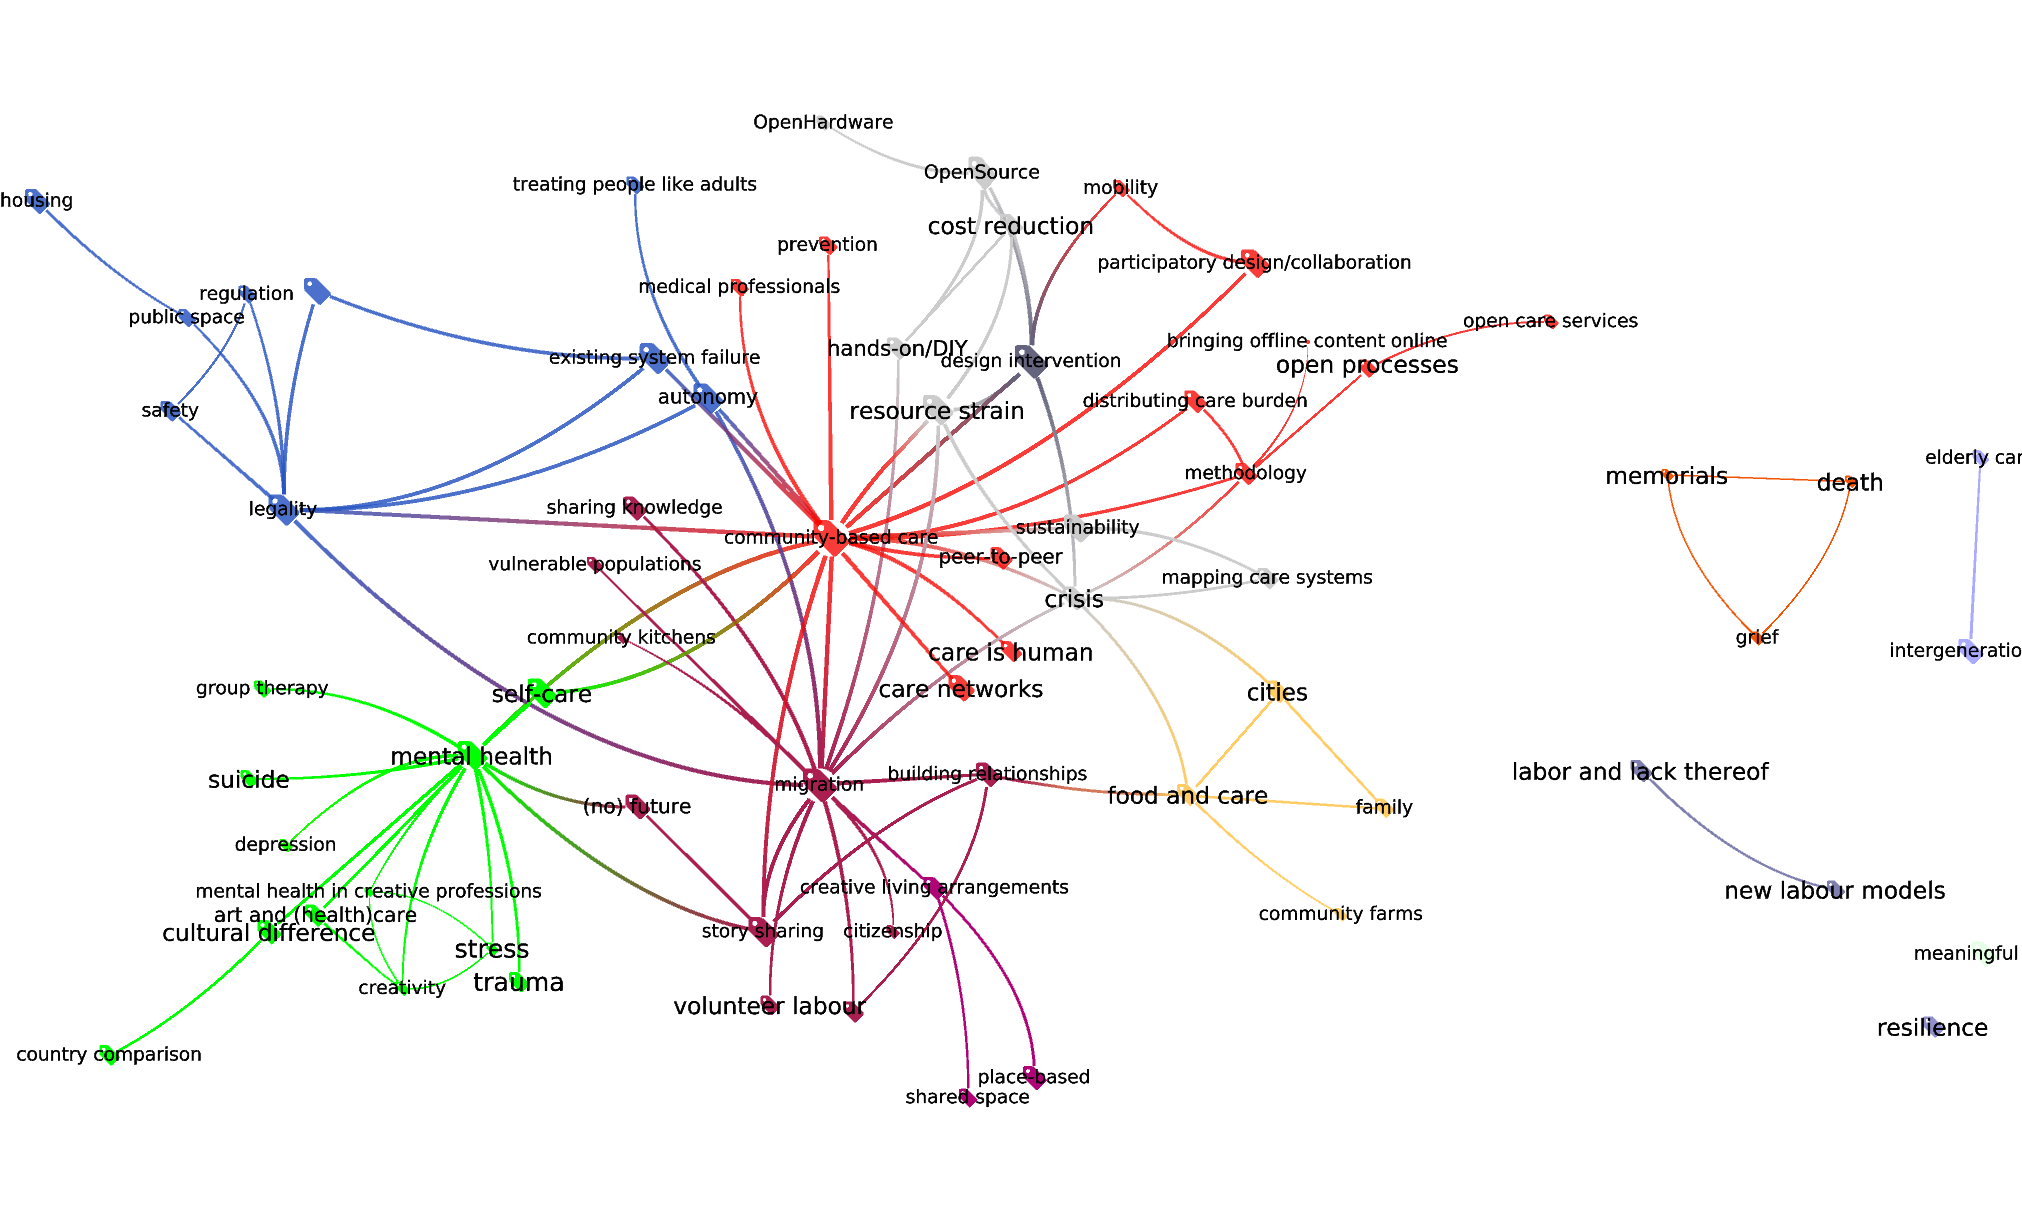
\includegraphics[scale=0.15]{images/edgeForce4.png}
\caption{The OpenCare code co-occurrence network (filtered for $k>=5$).}
\label{fig:NetViz}
\end{figure}

\subsection{Exploring the co-occurrence network for novelty} \label{ssec_exploring_novelty}

% The co-occurence network gives both ethnographers who have spent extended time with the primary data and researchers without time to sift through that data new insights. Looking at the co-occurrence network at a high level (with edges with number of co-occurrences k<5 filtered out), allows researchers to explore connections that the community has deemed important by interacting around them extensively. For example, one section of the co-occurrence network, illustrated in green, clusters around the code “mental health.” Even without reading the associated stories, it is clear that the community has connected mental health to creativity, art and health care, story sharing, trauma and community-based care. Since the weak edges are filtered out, we know that there have been extended conversations around these issues. 

% From a cursory reading of the Open Care posts, without looking at the co-occurrence network, one might read a few stories about trauma emerging from migration and assume that mental health was largely being discussed in relation to refugees’ struggles. A simpler aggregation like a word cloud would also offer a similar top-level view, since migration and mental health are both discussed at length across the platform. From the co-occurrence network, however, we see that mental health issues span a range of contexts: labour issues, young people’s feelings of futurelessness, cultural difference, and stress, to name a few. 

% The network, however, does not just give us an idea of problems and their causes. It also suggests potential solutions to these issues. While self-care is an important theme, since existing health and social care systems have failed many community members, most of the solutions, as evidenced by mental health’s strong connection with the code “community-based care,” are community-based. The data tells us that for many, reaching out to others for care, support, and ideas provides vital relief from mental health issues. Looking at the co-occurrence network, it also becomes clear that there is a powerful link between creative expression and mental well-being. From these links we learn that for community members, trained professionals provide only one aspect of mental healthcare. In dealing with trauma especially, connecting people in different places, sharing support and resources, has been crucial. Technological solutions, as we can see from the data, also revolve around community-based care: platforms for bringing people together and enabling them to share knowledge, stories and resources. All of these observations come through at the level of the co-occurrence network, since solutions are visibly linked to problems.

Connections that spark interest can be explored at a more granular level, either by focusing on lower-$k$ co-occurrences between a chosen code and others (not shown), or by reading the original stories and posts in which the co-occurrences took place. Around  \texttt{mental health}, \texttt{stress} and \texttt{trauma},  one finds the specific (often low-cost and social) tools that people use to manage stress, for example, learning about the usefulness of \texttt{group therapy} and online support groups, alternative therapies like \texttt{holistic healthcare}, or simply \texttt{getting outdoors}. The method allows for rich analysis on multiple levels, and never loses the granularity that makes ethnographic research so powerful. 

Even at high levels, meaning comes through clearly and, crucially, high level connections illuminate connections that would be invisible at a smaller scale of analysis (for example the high-$k$ connections between \texttt{mental health} and \texttt{trauma}, and \texttt{creativity}, \texttt{art and health care}and \texttt{story sharing}. In OpenCare, for example, these high-level connections made visible by the co-occurrence graph have enabled us to theorise that people are each other's healthcare technologies, and we have been able to detail and verify that theory through engagement with the granular details present in the stories. Without the co-occurrence network, vital interconnections would have been missed; without the detailed ethnographic data, the meaning behind those connections would be lost. 


\section{Extensions and future research} \label{sec:extensions}

\subsection{Open data and large-scale collaboration in ethnography}

Social Semantic Networks hold the potential to make ethnography a large-scale collaborative discipline. For this to happen, we propose ethnographers embrace the practice of using and publishing open data. Open data are data that are (a) machine-readable, (b) published under licenses that allow their re-use, and (c) documented with appropriate metadata\footnote{We have done this with OpenCare: \url{https://doi.org/10.5281/zenodo.164970}; \url{https://github.com/opencarecc/opencare-data-documentation}}. This paves the way for:

\begin{enumerate}
\item \emph{Replication}. An ethnographer could pull in a colleague's primary and secondary data and check that the latter's process is clear. This increases the accountability of the research process.
\item \emph{Large scale studies}. Accurate documentation of the code ontology allows ethnographers to work consistently on projects that would be too large for a single ethnographer to tackle. This would allow ethnographic studies at the scale of the thousands of informants. 
\item \emph{Multilingual studies}. The code ontology can be structured as a hierarchy, so that codes with the same meaning in different languages are entered in the secondary data as children of the same parent code. For example, \texttt{labour} could have \texttt{travail} and \texttt{arbeit} as children. The code co-occurrence network would be drawn between parent nodes, thus allowing both an all-languages view on data and across-languages comparisons. 
\item \emph{Reuse and extension}. An ethnographer could pull in a colleague's primary and secondary data, add her own coded corpus and use the combination of annotated corpora to produce a completely new study – for example on responding to the refugee crisis, one of the care issues taken up by the OpenCare community. 
\item \emph{"Longitudinal ethnography"}. An online conversation could be revamped over time (for example every year) to keep track of how its collective point of view evolves. 
\end{enumerate}

The combination of these elements requires a cultural shift from practitioners. Ethnographers tend to work alone, and there is as yet no culture of open data in the discipline, as access to coded interviews and fieldnotes belongs to the ethnographer alone. To the best of our knowledge, the OpenCare dataset is the first-ever open dataset including primary and secondary data. 

Yet, the payoff of such a shift is substantial. Ethnography could bring its unique methodological advantages to new  problems, that demand a scale and consistency it now cannot supply. For example, we could imagine a version of Eurobarometer based on an open online conversation. Instead of answering multiple choice questions (vulnerable to framing biases~\cite{tversky1985framing}, informants would discuss their perception of Europe, allowing researchers to discover novel patterns of association and detect the fading of old ones.

\subsection{Other methodological improvements}

In the future, we plan to test with at least three improvements:

\begin{enumerate}
\item Weighing contributions (and consequently annotations) by a "reliability score" derived by applying social theory on the social network topology \cite{Burt2005}.
\item Applying alternative ways to measure edge (association) strength $k$ in the co-occurrence network; for example, $k(A \rightarrow B)$ could encode the number of informants that have authored contributions coded with both codes $A$ and $B$, or the number of separate threads which contain at least one contribution with it, and so on. Different measures of edge strength have different interpretations, so they would allow different perspectives on the data corpus. 
\item Observing and modelling the online conversation as a dynamic system. Stochastic Actor-Oriented Models might be a good place to start, despite known limitations (\cite{snijders1996stochastic}).
\end{enumerate}

\section{Conclusions}

Semantic social networks show some promise as a method for social research aimed at capturing collective intelligence (\cite{levy1997collective}, with some of the advantages of both purely qualitative traditional ethnography and quantitative surveys. Like traditional ethnography (but unlike surveys), they deal well with open questions and novelty. Like surveys (but unlike traditional ethnography), they can handle hundreds of informants. When combined with open standards and open data, they could perhaps attempt to handle thousands of informants. We look forward to exploring this potential further.


%\begin{table}[t]
%\centering
%\begin{subtable}[h]{0.55\textwidth}
%\centering
%  \begin{tabular}{|l | c |}
%  \hline
%  Tag label & Degree \\ \hline\hline
%  community-based care & 294 \\ \hline
%  migration & 252 \\ \hline
%  design intervention & 242 \\ \hline
%  legality & 207 \\ \hline
%  existing system failure & 205 \\ \hline
%  resource strain & 197 \\ \hline
%  autonomy & 194 \\ \hline
%  story sharing & 192 \\ \hline
%  self-care & 187 \\ \hline
%  mental health & 186 \\ \hline
%  \end{tabular}
%  \caption{Opencare tag network}
%\end{subtable}\hfill
%\begin{subtable}[h]{0.4\textwidth}
%\centering
%  \begin{tabular}{|l | c |}
%  \hline
%  Tag label & Degree \\ \hline\hline
%  lakedistrict & 307 \\ \hline
%  cumbria & 302 \\ \hline
%  nature & 296 \\ \hline
%  photooftheday & 276 \\ \hline
%  england & 271 \\ \hline
%  love & 270 \\ \hline
%  doncaster & 248 \\ \hline
%  yorkshire & 233 \\ \hline
%  fitness & 219 \\ \hline
%  instagood & 190 \\ \hline 
%  \end{tabular}
%  \caption{Instagram dataset}
%\end{subtable}
%\vspace{-5pt}
%\caption{Top 10 tags ordered by degree for each dataset.}
%%\vspace{-20pt}
%\label{tab:degree}
%\end{table}
%
%With our two datasets gathered using respectively SMT and EC, we observe, analyse and compare them in order to find disparities occurring on one side but not on the other. To this end, we start by looking at the ten most popular tags for both co-occurrence graphs based on the degree, as shown in Table~\ref{tab:degree}. As one can see and expect due to their degree distribution being on par of scale-free networks, very few nodes possess a high degree. Other than that, the tags encountered are not unexpected considering the context of both graphs, with OC tags revolving around health and social care while Instagram's are largely descriptive in nature and  mention locations (e.g., \texttt{lake district}, \texttt{cumbria}, \texttt{doncaster}, \texttt{yorkshire}, \texttt{nature}, \texttt{england}), photo, fitness and food.
%
%A more surprising result appears however when glancing at the co-occurrences between two tags, and more particularly, which two tags often appear one with another. We show in Table~\ref{tab:co-occ} such results detailing the five most common pairs of tags for each dataset. Aside from the great difference between the number of co-occurrences (C) encountered for each pair due to the number of messages existing in the respective initial datasets, we realise that unlike the co-occurring relations returned by OC which are mostly between the most popular tags, Instagram's do not follow the same pattern.
%
%The co-occurrences in OC have established meanings. When placed side-by-side, some of the pairs begin to outline problems, for instance linking together the \texttt{legality} issues or \texttt{ressource strain} arising along \texttt{migration} or \texttt{community-based care}. Nonetheless, the pairs also often hint at potential solutions to those problems. Thus, issues of \texttt{legality} are addressed with solutions \texttt{outside existing systems}, some \texttt{migration} problems can be worked out by \texttt{building relationships} with the local, and \texttt{mental health} can be bettered by \texttt{creativity} and \texttt{art and care}.
%
%In the case of the Instagram dataset however, aside from the pair formed by the very well connected tags \texttt{cumbria} and \texttt{lakedistrict}, the remaining co-occurring tags are not among the twenty most used tags. They actually originate from a barbershop/tatoo parlor in Bawtry, called The Gentleman's Retreat, with a very successful viral marketing campaign (\texttt{tgr}, \texttt{thegentlemansretreat}, \texttt{barberlife}) also used to promote hair products (\texttt{apothecary87}, \texttt{themanclub}). While only a limited number of elements is show in Table~\ref{tab:co-occ}, the tendency is not a mere artifact and goes beyond the first few elements and well into the first twenties. It is a good example showing one of the possible outcome likely to appear when using user-generated tags.
%
%\begin{table}[t]
%\centering
%\begin{subtable}[h]{0.5\textwidth}
%\centering
%  \begin{tabular}{|l | c |}
%  \hline
%  Tag -- Tag label & C \\ \hline\hline
%  migration -- build. relationships & 11 \\ \hline 
%  comm.-based care -- legality & 10 \\ \hline 
%  migration -- res. strain & 10 \\ \hline 
%  res. strain -- comm.-based care & 9 \\ \hline 
%  legality -- migration & 9 \\ \hline 
%  existing system failure -- legality & 9 \\ \hline 
%  migration -- story sharing & 9 \\ \hline 
%  safety -- regulation & 9 \\ \hline 
%  mental health -- creativity & 9 \\ \hline 
%  mental health -- art and care & 8 \\ \hline 
%  \end{tabular}
%  \caption{Opencare tag network}
%\end{subtable}\hfill
%\begin{subtable}[h]{0.5\textwidth}
%\centering
%  \begin{tabular}{|l | c |}
%  \hline
%  Tag -- Tag label & C \\ \hline\hline
%  cumbria -- lakedistrict & 277 \\ \hline 
%  thegentlemansr. -- bawtry & 188 \\ \hline 
%  bawtry -- barbershop & 183 \\ \hline 
%  thegentlemansr. -- barbershop & 183 \\ \hline 
%  bawtry -- themanclub & 181 \\ \hline 
%  thegentlemansr. -- themanclub & 181 \\ \hline 
%  themanclub -- barbershop & 177 \\ \hline 
%  bawtry -- apothecary87 & 172 \\ \hline 
%  thegentlemansr. -- apothecary87 & 172 \\ \hline 
%  themanclub -- apothecary87 & 171 \\ \hline 
%  \end{tabular}
%  \caption{Instagram dataset}
%\end{subtable}
%\vspace{-5pt}
%\caption{Top 10 pair of tags often appearing together ordered by the number of co-occurrences (C).}
%\label{tab:co-occ}
%\end{table}
%
%There are a few structural differences that must be noted between the two datasets. Firstly, Instagram is a photo sharing site which is not truly oriented toward any particular purpose, whereas OpenCare is geared toward story sharing around a specific topic. In this sense, while participants on both platforms are self-selected, OpenCare users already care in some way or another about the topic at hand and thus will orient the discussion toward health care related topics. Second, while we only preserve the tags/hashtags for each posts and ignore the rest, we miss textual information from both datasets but also the visual data inherently linked to the Instagram posts, since the primary contribution of Instagram users is their photos. 
%Nonetheless, while social media trawling is a very quick and easy solution to obtain annotated data, the user-generated tags are proposed and affected by non-experts, thus lacking the consistency and overall quality of annotations proposed by ethnographers.
%
%Despite that, one would expect larger data to be a proper guarantee where the quantity of content could end up correcting any irregularities in the attribution of tags, however, this is only true as long as the number of people performing irregularities in the network, like responding or helping viral marketing, is kept to a minimum. We see however that, for the same analysis, annotations of quality with cohesive and stable appellations return much more concording results, marking the intervention of the ethnographer a worthwhile investment.
%
%
%%We have proposed in this paper a comparison between two datasets gathered using distinct online ressources. Whereas the first dataset in based on the well known social media platform Instagram, the second uses a much smaller online forum populated by health and social care enthusiasts. While the first population is larger and generate a lot of content, the second group is very specialised a only discuss about specific topics. We have used two very different approaches to study the datasets, the first one relying on user-generated annotations and the second using professional ethnographic annotations to describe the discussion of the smaller network.


\paragraph{Acknowledgment}
The OpenCare project has received funding from the European Research Council (ERC) under the European Union's Horizon 2020 research and innovation program (grant agreement no 688670).

%
% ---- Bibliography ----
%
\bibliographystyle{plain}
\bibliography{biblio.bib}
\end{document}

\subsection{Differences in network structure} \label{ssec_network_structure}

(The text here is meant to share results, it is not what we intend to write.) 

First, I report values gotten from fitting the plain degree distribution.

\begin{itemize}
\item OC
	\begin{itemize}
	\item fit.power\_law.alpha = 3.2328951624984361
    \item fit.power\_law.sigma = 0.19217701729296771 (Alberto can probably tell what this sigma is)
    \item fit.xmin = 55.0
    \item and when using xmin=1.0, fit.power\_law.alpha = 1.3948927229745787
	\end{itemize}
\item IO
	\begin{itemize}
	\item fit.power\_law.alpha = 2.977553767058077
    \item fit.power\_law.sigma = 0.13393684157206664
    \item fit.xmin = 44.0
    \item and when using xmin=1.0, fit.power\_law.alpha = 1.3641779299784778
	\end{itemize}
\end{itemize} 

Second, I report values gotten from fitting the weighted degree distribution.

\begin{itemize}
\item OC
	\begin{itemize}
	\item fit.power\_law.alpha = 2.7656794024195568
	\item fit.xmin = 60.0
    \item and when using xmin=1.0, fit.power\_law.alpha = 1.3795264972632906
	\end{itemize}
\item IO
	\begin{itemize}
	\item fit.power\_law.alpha = 2.0427986581473614
    \item fit.xmin = 66.0
    \item and when using xmin=1.0, fit.power\_law.alpha = 1.2320308193590144
	\end{itemize}
\end{itemize} 

\emph{Does that show significant differences?}

---

nontrivial social network\footnote{It can, of course, induce trivial ones. For example, one could impose that all informants posting in a certain local authority are connected, but this would induce very large cliques with very little information content. Alternatively, one could track a "real" conversation network in Instagram; this is done through tracking mentions of each user $i \in N$ by all users $j \neq i  \in N$. The authors of the Instagram study did not attempt this; we conjecture it would result in a very sparse network, again with very little information content.}. What informants have in common is that they happened to be posting on Instagram in a certain period in 2015, and they were in certain areas when they did so.

Looking at the data, and here is one thing that may be worth underlining as a major structural difference between the two networks. The single core structure I am guessing here is best emphasized when looking at the $k$-core and weighted $k$-core statistics.

\begin{itemize}
\item Compute both plain $k$-core (based on plain degree) and weighted $k$-core.
\item Also, assign edges a k-core index (that k value occurring when the edge vanishes).
\item OC seems to have a single core around which the whole network is built. This is how I interpret the lower modularity values we get for OC compared to IO.
\end{itemize}

\begin{figure}[!h]
\begin{center}
\includegraphics[scale=0.25]{images/kcore_OC.png}
\end{center}
\caption{Statistical distribution of the unweighted and weighted $k$-core statistics on OC.}
{\label{fig:kcore_OC}}
\end{figure}

\begin{figure}[!h]
\begin{center}
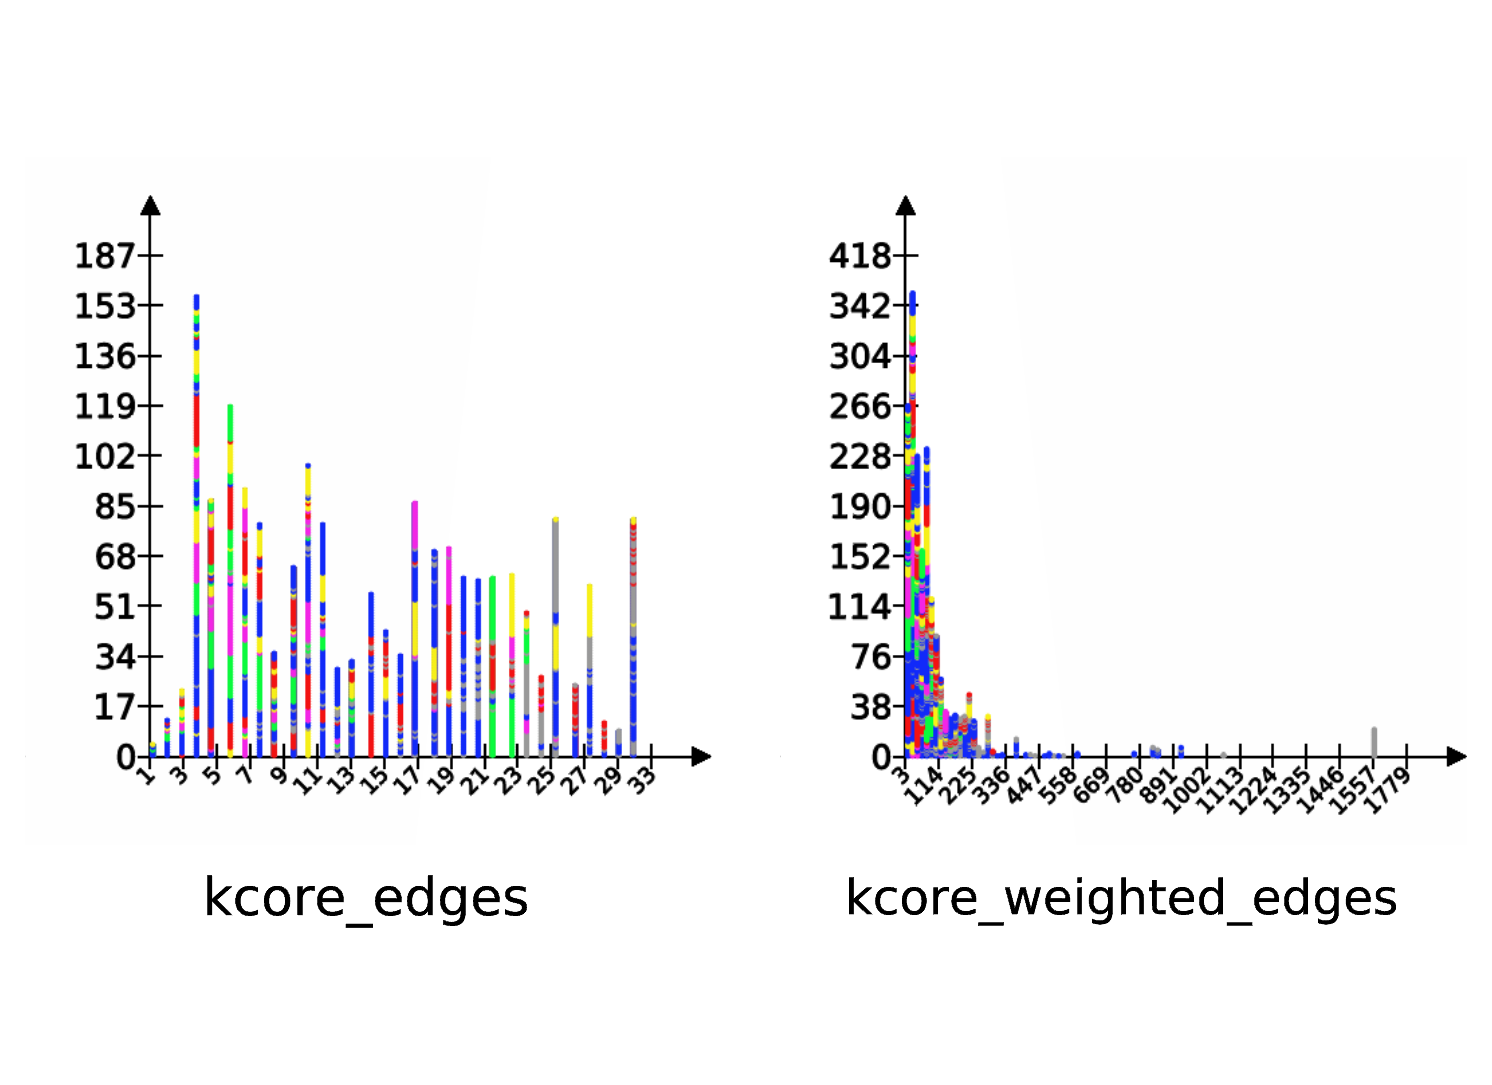
\includegraphics[scale=0.25]{images/kcore_IO.png}
\end{center}
\caption{Statistical distribution of the unweighted and weighted $k$-core statistics on IO.}
{\label{fig:kcore_OC}}
\end{figure}

Now, the maximum $k$ value when computing $k$-core on OC is 49, while it is only 32. That is, IO gets peeled off of its edges faster than OC does. This phenomenon is amplified when we consider the weighted $k$-core (using number of co-occurrences as edge weights). The Pearson correlation coefficient hits a 0.96 value for OC while IO only gets as high as 0.48. The shape of the distribution on OC for both $k$-core and weighted $k$-core are quite similar, while the weighted $k$-core for  IO clearly show a powerlaw distribution.

Additionally, the top 20 tags (ranked according to the weighted $k$-core statistics) differ, although they intersect the set of the top 20 more occurring tags. The top 20 weighted $k$-core tags for OC are listed here. Common tags are mark using boldface.

  \begin{tabular}{| l |}
  \hline
  Tag label  \\ \hline \hline
\textbf{youth} \\ \hline
working with policy makers \\ \hline
visibility \\ \hline
\textbf{design intervention} \\ \hline
turning desires into solutions \\ \hline
trust \\ \hline
treating people like adults \\ \hline
(no) future \\ \hline
accessibility \\ \hline
definition of community \\ \hline
anti-racist \\ \hline
art and (health)care \\ \hline
third sector organizations \\ \hline
technology \\ \hline
systems-based vs family-based care \\ \hline
\textbf{sustainability} \\ \hline
support system \\ \hline
\textbf{story sharing} \\ \hline
\textbf{autonomy} \\ \hline
\textbf{skill sharing} \\ \hline
  \end{tabular}

The top 20 weighted $k$-core tags for IO are:

  \begin{tabular}{| l |}
  \hline
  Tag label  \\ \hline \hline
beer \\ \hline
ale \\ \hline
craftbeerlover \\ \hline
craftbeernotcrapbeer \\ \hline
beergasm \\ \hline
beerpremiumale \\ \hline
beerisculture \\ \hline
hophead \\ \hline
beergeek \\ \hline
beertography \\ \hline
instabeerofficial \\ \hline
boozethread \\ \hline
beerlover \\ \hline
craftnotcrap \\ \hline
instabeer \\ \hline
craftbeerdrinker \\ \hline
beernerd \\ \hline
carryonale \\ \hline
beersnob \\ \hline
realale \\ \hline
\end{tabular}

\subsection{Differences in semantics}

Comparing top tags and co-occurrences between OpenCare (OC) and Instagram obesity (IO) datasets, clear differences become apparent. IO tags (that do not reflect viral advertising campaigns) are largely descriptive in nature, referencing things like places: \texttt{\#lake district} + \texttt{\#cumbria}; \texttt{\#doncaster}; \texttt{\#yorkshire}; \texttt{\#nature}; \texttt{\#summer}. OC's top tags and co-occurrences, on the other hand, index more nuanced connections, and when placed side-by-side begin to outline problems and often potential solutions to those problems: \texttt{legality} + \texttt{outside existing systems}; \texttt{community-based care}; \texttt{migration} + \texttt{building relationships}; \texttt{mental health} + \texttt{creativity}. 

Let us take, for example, the co-occurrence of \texttt{legality} and \texttt{outside existing systems}. \todo{insert w/edits user pathway from https://edgeryders.eu/en/opencare-research/dashboard-demo-walkthrough-with-pictures to illustrate the capacity of the CE approach in OC}


\todo{This goes at the end of this subsection} There are a few structural differences that must be noted. Firstly, Instagram is a photo sharing site which is not oriented toward any particular purpose, whereas OpenCare is geared toward story sharing around a specific topic. In this sense, while participants on both platforms are self-selected, OpenCare users already care in some way or another about the topic at hand. Second, we miss large amounts of visual data when Instagram posts are reduced to hashtags, since the primary contribution of Instagram users is their photos. 





\begin{table}[h]
\centering
\begin{tabular}{|l | c |}
\hline
Edge co-occurrence & Edge\_force \\ \hline \hline 
migration - building relationships & 11 \\ \hline 
community-based care - legality & 10 \\ \hline 
migration - resource strain & 10 \\ \hline 
resource strain - community-based care & 9 \\ \hline 
legality - migration & 9 \\ \hline 
existing system failure - legality & 9 \\ \hline 
migration - story sharing & 9 \\ \hline 
safety - regulation & 9 \\ \hline 
mental health - creativity & 9 \\ \hline 
mental health - art and (health)care & 8 \\ \hline 
legality - safety & 8 \\ \hline 
crisis - resource strain & 8 \\ \hline 
regulation - legality & 8 \\ \hline 
mental health - suicide & 7 \\ \hline 
outside existing systems - legality & 7 \\ \hline 
cost reduction - design intervention & 7 \\ \hline 
mental health - trauma & 7 \\ \hline 
care networks - community-based care & 7 \\ \hline 
community-based care - peer-to-peer & 7 \\ \hline 
food and care - community farms & 7 \\ \hline
\end{tabular}\vspace{5pt}
\caption{Top 20 co-occurring tags ordered by frequence for the Opencare tag network.}
\end{table}

\section{Discussion} \label{sec_discussion}

\section{Remarks}
Following our email thread and Jason last comment.

Looking at the IO network, and at how tag co-occurrence and edge redundancy (Simmelian backbone~\cite{Nick2013}) behave.

\begin{figure}[!h]
\begin{center}
\includegraphics[scale=0.4]{images/nb_co_occur_redundancy_highest.jpg}
\end{center}
\caption{Scatterplot nb co-occur. / redundancy. Highlighting higher redundancy, higher weight.}
{\label{fig:scatterplot}}
\end{figure}

\begin{figure}[!h]
\begin{center}
\includegraphics[scale=0.4]{images/nb_co_occur_redundancy.jpg}
\end{center}
\caption{Scatterplot nb co-occur. / redundancy. Highlighting higher redundancy, lower weight.}
{\label{fig:scatterplot}}
\end{figure}

The edges connecting the ``viral marketing about the beards'' hashtags simultaneously hit the highest co-occurence *(weight — sic) *and* highest redundancy. Except for one edge linking « cumbria » and « lakedistrict ». Nodes connected by these edges do not however all fall in a same cluster.





\paragraph{Acknowledgment}The Opencare project has received funding from the European Union's Horizon 2020 research and innovation program under grant agreement No 688670.
%
% ---- Bibliography ----
%
\bibliographystyle{plain}
\bibliography{biblio.bib}
\end{document}
\begin{thebibliography}{5}

\bibitem{burt}
Burt, R. S. (2005). Brokerage and closure: An introduction to social capital. Oxford university press.

\bibitem{cottica:melancon}
Cottica, Alberto, Guy Melançon, and Benjamin Renoust. "Testing for the signature of policy in online communities." International Workshop on Complex Networks and their Applications. Springer International Publishing, 2016.

\bibitem{kleinberg}
Kleinberg, J. M. (1999). Hubs, authorities, and communities. ACM computing surveys (CSUR), 31(4es), 5.

\bibitem {munk:abilgaard}
Munk, Anders Kristian, et al. 
"(Re-) Appropriating Instagram for Social Research: Three Methods for Studying Obesogenic Environments." 
Proceedings of the 7th 2016 International Conference on Social Media \& Society. ACM, 2016.

\bibitem{rheingold}
Rheingold, Howard. "The virtual community: Homesteading on the electronic frontier." (2000).



\end{thebibliography}

\end{document}

% OC on tag main component (990n; 12,777e): CC: 0.71091, CPL: 2.58182, avg deg: 25.8121212121
%     regular ring lattice (990n; 12,870e): CC: 0.72   , CPL: 19.5197
%          ER random graph (990n; 12,870e): CC: 0.02686, CPL: 2.46629

% IO on tag main component (2045n; 23,693e): CC: 0.834336, CPL: 3.26446, avg deg: 25.8121212121
%     regular ring lattice (2045e; 24,540e): CC: 0.717391, CPL: 43.0841
%          ER random graph (2045e; 24,540e): CC: 0.011982, CPL: 2.73801
